%
% $RCSfile: composite.tex,v $
%
% Copyright (c) 2004. Christian Heller. All rights reserved.
%
% No copying, altering, distribution or any other actions concerning this
% document, except after explicit permission by the author!
% At some later point in time, this document is planned to be put under
% the GNU FDL license. For now, _everything_ is _restricted_ by the author.
%
% http://www.cybop.net
% - Cybernetics Oriented Programming -
%
% http://www.resmedicinae.org
% - Information in Medicine -
%
% @author Christian Heller <christian.heller@tuxtax.de>
%

\paragraph{Composite}
\label{composite_heading}

A hierarchical object structure, also called \emph{Directed Acyclical Graph}
(DAG) or \emph{Tree}, can be represented by a combination of classes called
\emph{Composite} pattern \cite{gamma1995}. It describes a \emph{Component} that
may consist of \emph{Children} (figure \ref{composite_figure}), which makes it
comparable to the \emph{Whole-Part} pattern. The difference is that the
\emph{Composite} is a more generalized version, with a dynamically extensible
number of child (part) objects.

The \emph{Composite} is a pattern based on \emph{Recursion}, which is one of
the most commonly used programming techniques at all. The pattern's split into
\emph{Leaf-} and \emph{Composite} sub classes helps distinguish primitive- from
container objects. A composite tree node holds objects of type \emph{Component}.

\begin{figure}[ht]
    \begin{center}
        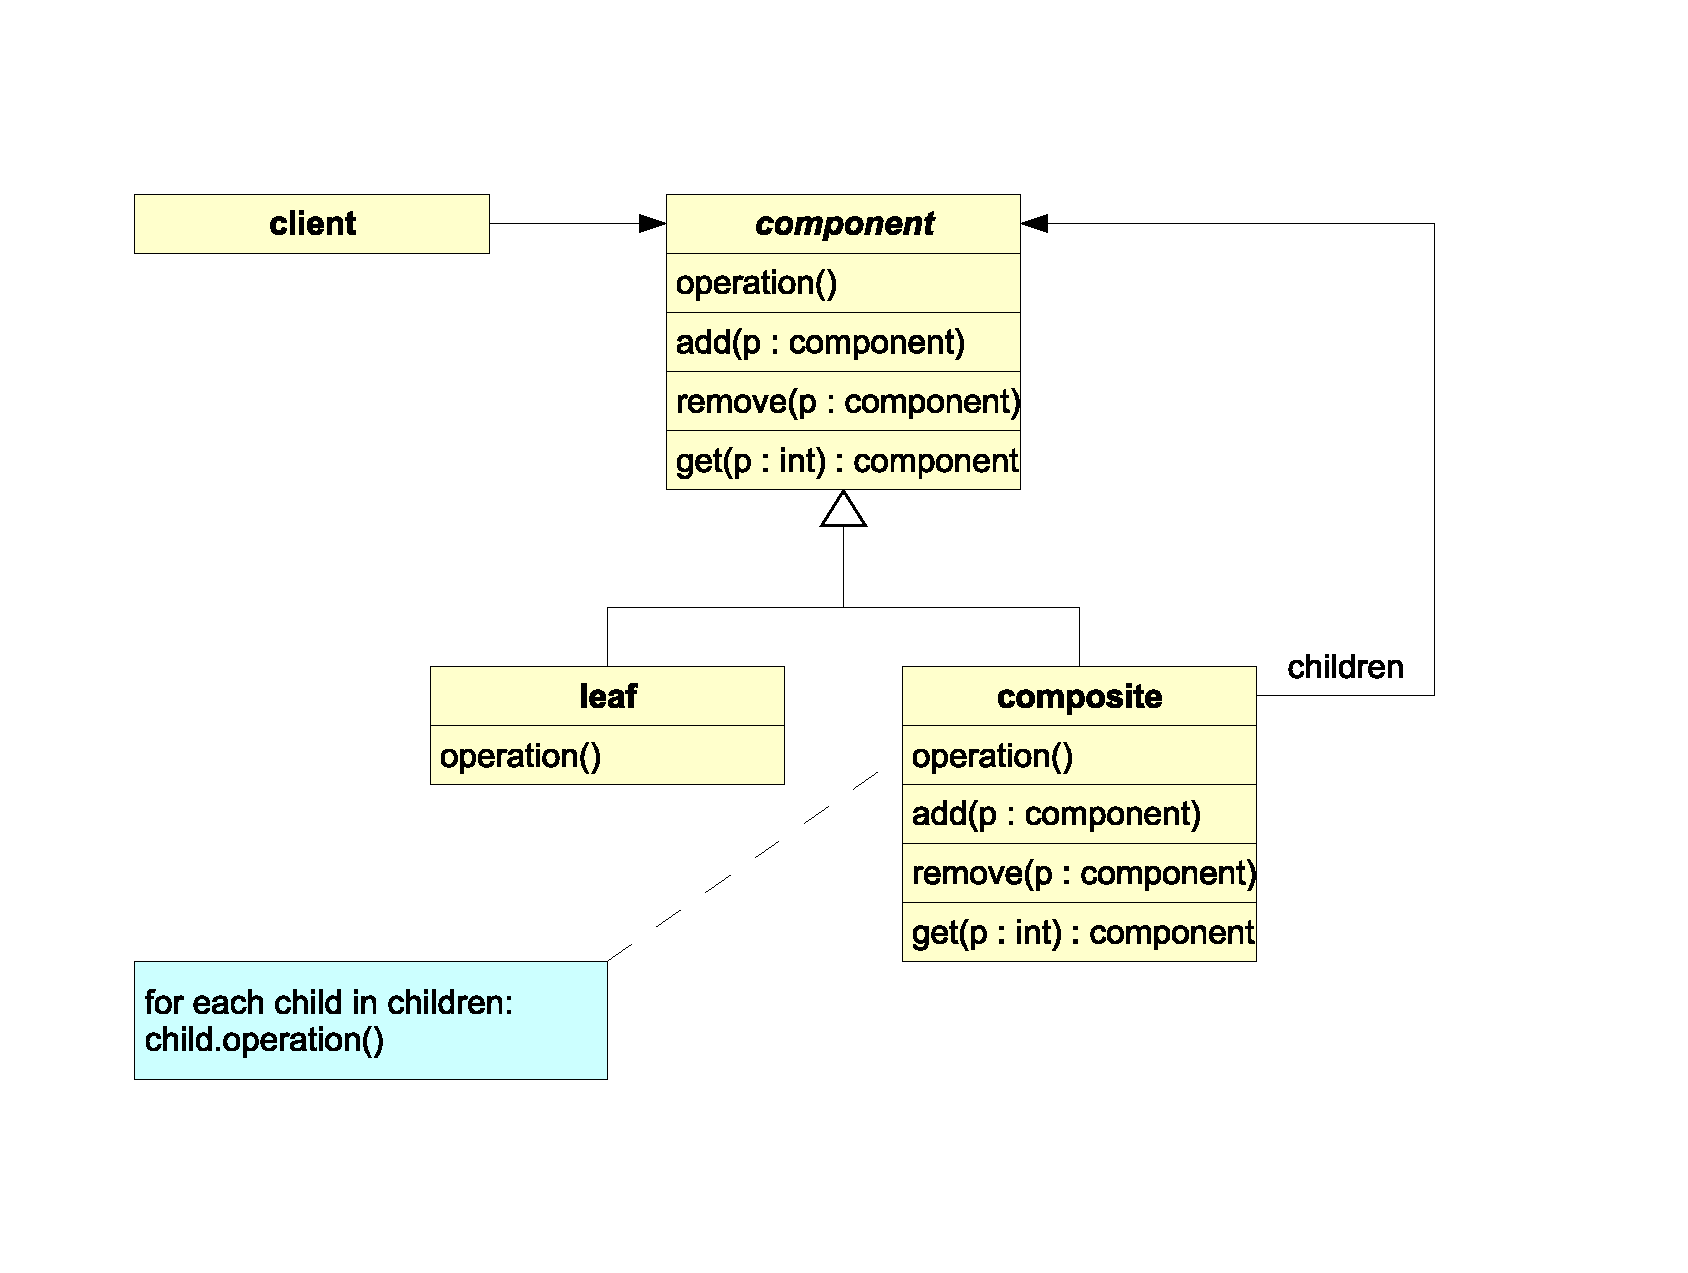
\includegraphics[scale=0.3]{vector/composite.eps}
        \caption{Composite Pattern}
        \label{composite_figure}
    \end{center}
\end{figure}
